\section{Bibliothek zur visuellen Darstellung insbesondere von Graphen}

Nachdem die theoretischen Visualisierungsmethoden der bestehenden Literatur nun abschließend erläutert worden sind, wird nun eine Bibliothek für die Implementation der Darstellung von Graphen vorgestellt. \emph{Cytoscape} ist eine Bibliothek für auf JavaScript-basierende Applikationen, welche die Erstellung eines Graphen im Frontend wesentlich erleichtert. Häufig wird Cytoscape für biologische Prozesse und Zusammenhänge verwendet, da besonders diese natürlichen wissenschaftlichen Bereiche ähnliche Strukturen wie Graphen aufweisen. Ursprünglich ist Cytoscape auch für genau diese Zwecke an der \wordindoublequotes{University of Toronto} entwickelt und anschließend in \wordindoublequotes{Oxford Bioinformatics} publiziert worden. Die Anwendungsbereiche von Graphenvisualisierungen gehen jedoch weit über den biomolekulare Bereich hinaus. \cite{Cytoscape}

Cytoscape bringt einige Vorteile mit sich. Die Bibliothek ist einfach zu verwenden und verfügt über eine detaillierte Dokumentation. Darüberhinaus gibt es inspirierende Demonstrationen, wie die Bibliothek verwenden werden kann. Diese Beispiele haben bei der Implementierung des Prototypen sehr geholfen. \cite{Cytoscape}

Bemerkenswert an Cytoscape ist auch das Eco-System und die Community, da es nicht nur viele Plugins, sprich Erweiterungen, gibt, sondern auch eine Variation an unterstützen Modulsystemen, darunter \wordindoublequotes{ES modules}, \wordindoublequotes{Node.js} und \wordindoublequotes{AMD/Require.js}. Des Weiteren wird Cytoscape in allen modernen Browsern unterstütz -- eine extrem wichtige Eigenschaft für Frontend-Developer heutzutage. Und genau das sind auch einige der Gründe, warum wir uns für die Verwendung der Bibliothek Cytoscape entschieden haben. \cite{Cytoscape}

Alle Vorteile und Eigenschaften von Cytoscape sind nochmals übersichtlich in Abbildung \ref{fig:CytoscapeArchitektur} dargestellt.

\begin{figure}
    \centering
    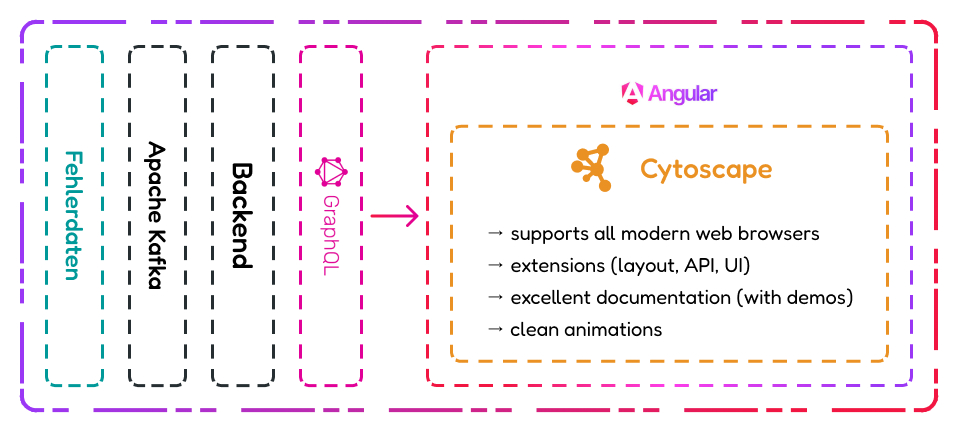
\includegraphics[width=1\textwidth]{content/img/Architecture/Architecture_Cytoscape.jpg}
    \caption{Architektur unseres Prototypen mit Fokus auf die Bibliothek Cytoscape}
    \label{fig:CytoscapeArchitektur}
\end{figure}
\FloatBarrier

Die Darstellungen anderer Grafiken, wie Beispielsweise Diagramme, verwenden jeweils entsprechend passende Bibliotheken. \emph{ng2-charts} eignet sich besonders gut für das Darstellen von Diagrammen in Angular Applikationen und basiert auch der allgemeinen JavaScript Bibliothek für Diagramme, \emph{Chart.js}. \cite{ng2-charts}